\documentclass[a4paper]{report}
\usepackage{RJournal}
\usepackage{graphicx}
\usepackage{url}
\usepackage{amssymb}
\usepackage{amsmath}
\usepackage{verbatim}
\usepackage{tikz}
\usepackage{rotating}
\usepackage[round]{natbib}

\usetikzlibrary{positioning,petri}

%\SweaveOpts{width=6,height=4}

%\VignetteIndexEntry{Multiple table data in R}
%\VignettePackage{multitable}
%\VignetteDepends{multitable, MASS, lattice}
%\VignetteKeywords{data manipulation, ecology, multivariate, R}

%\usepackage{Sweave}
\begin{document}
\begin{article}
\title{Multiple-table data in \R}
\author{by Steven C Walker, Guillaume Gu\'{e}nard, and Pierre Legendre}
\maketitle

 



%% redefine some print methods to make better output on sweave

\abstract{Data frames are integral to \R.  They provide a standard format for passing data to model-fitting and plotting functions, and this standard makes it easier for experienced users to learn new functions that accept data as a single data frame.  Still, many data sets do not easily fit into a single data frame.  Manipulating such inherently multiple-table data using several data frames can result in long and difficult-to-read workflows.  We introduce the \pkg{multitable} package to provide new data storage objects called \code{data.list} objects, which extend the \code{data.frame} concept to explicitly multiple-table settings.  Like data frames, data lists are lists of variables stored as vectors; what is new is that these vectors have dimension attributes that make accessing and manipulating them easier.  As \code{data.list} objects can be coerced to \code{data.frame} objects, they can be used with all \R\ functions that accept an object that is coercible to a \code{data.frame}.}

\section{Introduction}

The standard data management paradigm in \R\ is based on \code{data.frame} objects, which are two-dimensional data tables with rows and columns representing replicates (sometimes also called objects) and variables.  Standard \R\ workflows require that the data to be analysed are organised into a data frame \citep{ChambersAndHastie1992}.  Hypotheses about the relationships between variables in the data frame are expressed using \code{formula} objects.  Data frames and formulas are combined by passing them to functions that produce analyses (e.g. plots; fitted models; summary statistics).  This framework allows scientists to concentrate on their primary interests---the relationships between variables---without explicit reference to mathematical and algorithmic details.  It also provides access to those details, which are required for more effective analyses and to develop new methods of analysis within the framework.  As new methods are developed, researchers simply pass their data frames to new functions in much the same way they would pass them to older functions.  Thus, by separating low-level methods development from high-level data analysis, \R\ fosters the formation of a community of researchers where both methodologists and analysts have mutually beneficial interactions.

Research in community ecology (i.e. the ecology of more than one species) sometimes involve data sets that do not easily fit within a single data frame.  A common example is the fourth-corner problem \citep{LegendreEtAl1997}, in which three data tables are to be analysed: a sites-by-species table of abundances or occurrences; a table of environmental variables at each site; and a table of traits for each species (Fig. \ref{fig:fourth}).  Such data are characterised by a conspicuous (lower-right) `fourth-corner', where there are no data.  The missing data in the fourth corner are not caused by the usual problems (e.g. broken field equipment; budget restrictions; bad weather; dead subjects), but are part of the study design itself.  The fourth-corner problem is a special case of a general `multiple-table problem', which can be much more complex (e.g. could involve three-dimensional `cubes' of data, Fig. \ref{fig:beatrix}).  The challenge of analysing such multiple-table data sets in \R\ is that it is not obvious how to organise them into a single \code{data.frame}, which is required in standard \R\ workflows.  Our goal with the \pkg{multitable} package is to provide tools that make analysing multiple-table data sets easier.

\begin{figure}
\vspace{0.5cm}
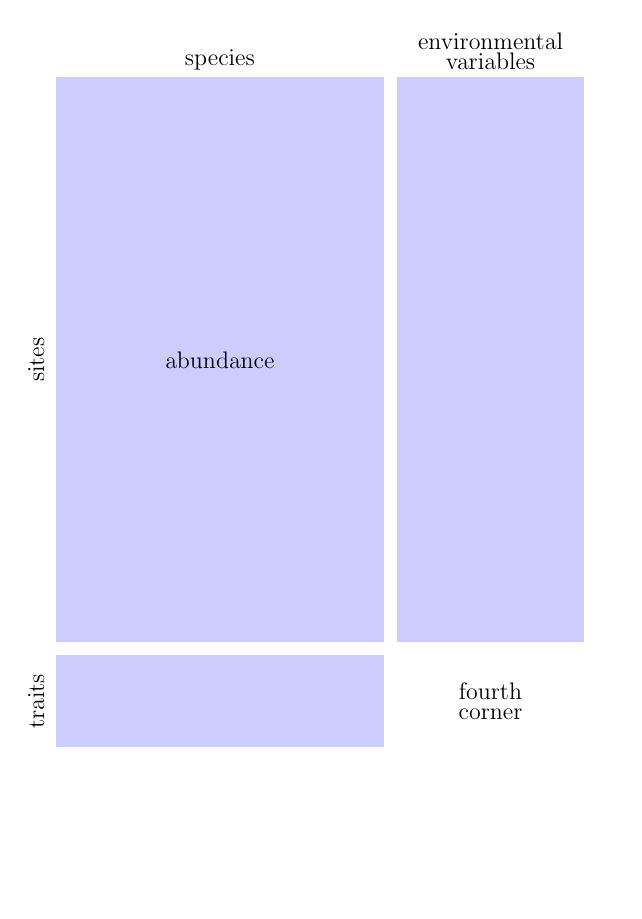
\begin{tikzpicture} [
	% transform shape makes scale 'work'
	scale=0.6, transform shape, 
	text centered,
	node distance=0.2cm,
	Y/.style={
		rectangle,draw=blue!0,fill=blue!20,thick,
		minimum width=7cm,minimum height=12cm,
		label=above:\Large species},
	X/.style={
		rectangle,draw=blue!0,fill=blue!20,thick,
		minimum width=4cm,minimum height=12cm,
		label={
		[text width=5cm]above:\Large environmental variables
		}},
	Z/.style={
		rectangle,draw=blue!0,fill=blue!20,thick,
		minimum width=7cm,minimum height=2cm},
	C/.style={
		rectangle,draw=red!0,fill=red!0,thick,
		minimum width=4cm,minimum height=2cm,
		text width=2cm},
	nm/.style={rectangle,minimum height=8cm,
	minimum width=0cm,draw opacity=0}
	]
\node [place,Y] 		(com)			{\Large abundance};
\node [place,X]	 	(env)[right=of com]	{};
\node [place,Z] 		(trt)[below=of com]	{};
\node [place,C]		(fc)[right=of trt]		{\Large fourth corner};
\node [place,nm]	(anm)[left=of com]	{\begin{turn}{90}
									\Large sites
								\end{turn}
								};
\node [place,nm]	(tnm)	[left=of trt]		{\begin{turn}{90}
									\Large traits
								\end{turn}
								};
\end{tikzpicture}
\vspace{-1.5cm}
\caption{Schematic diagram of a data structure with a fourth-corner problem.} 
\label{fig:fourth}
\end{figure}

One possible solution is to develop new \R\ analysis functions---or new software packages altogether---that are specifically designed to accept several tables as input.  There have been several such methods developed in ecology, focusing on data with a fourth-corner problem \citep{DoledecEtAl1996,LegendreEtAl1997,DrayAndLegendre2008,PillarEtAl2010,LeiboldEtAl2010,IvesAndHelmus2011}.  However, these methods do not apply to data sets that have other more complex multiple-table data structures (e.g. zooplankton communities in Lac Croche, Fig. \ref{fig:beatrix}) \citep{CantinEtAl2011}.  One approach to such issues would be to develop suites of data analysis functions for each new data structure.  But such an approach is less than ideal, as it would require that new methods be developed for each new structure---it does not take advantage of the large number of tools developed for standard \R\ workflows \citep{ChambersAndHastie1992}.  The \pkg{multitable} package provides an alternative approach, by introducing a multiple-table generalisation of data frames---called data lists---which can be analysed with virtually any function that can be used to analyse a data frame.  Thus, instead of providing new methods of analysis, \pkg{multitable} provides new methods of data management and organisation.

\begin{figure}
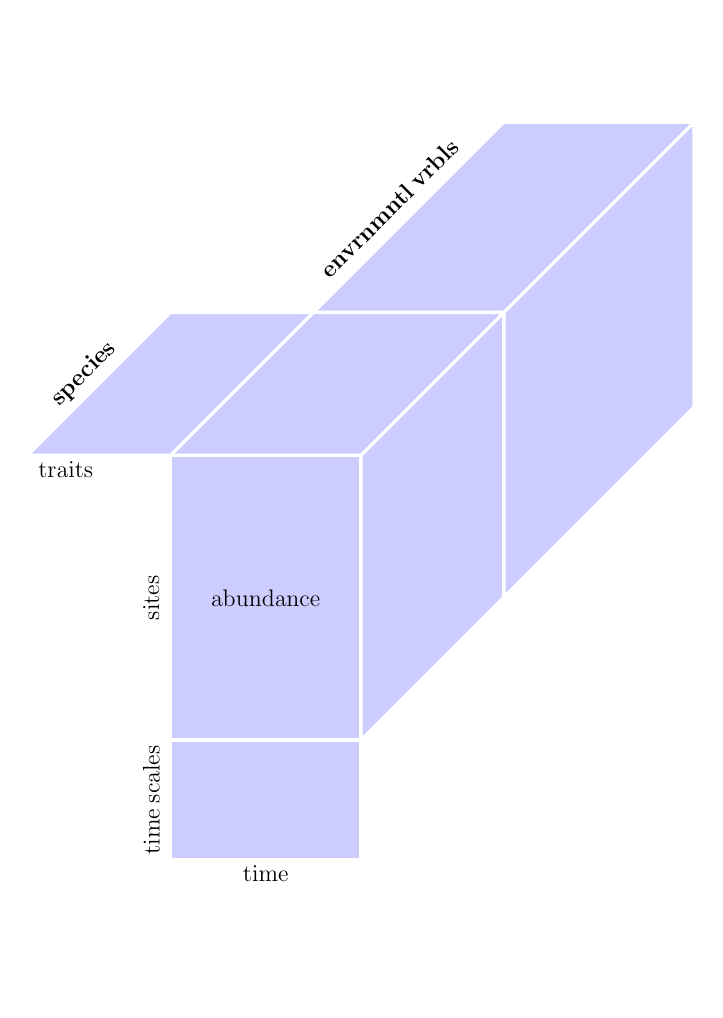
\begin{tikzpicture} [
	% transform shape makes scale 'work'
	scale=0.6, transform shape, 
	text centered,
	node distance=0cm,
	yfront/.style={
		rectangle,draw=blue!0,fill=blue!20,thick,
		minimum width=4cm,minimum height=6cm},
	time/.style={
		rectangle,draw=blue!0,fill=blue!20,thick,
		minimum width=4cm,minimum height=2.5cm,
		label=below:\Large time},
	ytop/.style={
		rectangle,draw=blue!0,fill=blue!20,thick,
		minimum width=4cm,minimum height=3cm,
		xslant=1},
	xtop/.style={
		rectangle,draw=blue!0,fill=blue!20,thick,
		minimum width=4cm,minimum height=4cm,
		xslant=1},
	yside/.style={
		rectangle,draw=blue!0,fill=blue!20,thick,
		minimum width=3cm,minimum height=6cm,
		yslant=1},
	xside/.style={
		rectangle,draw=blue!0,fill=blue!20,thick,
		minimum width=4cm,minimum height=6cm,
		yslant=1},
	trts/.style={
		rectangle,draw=blue!0,fill=blue!20,thick,
		minimum width=3cm,minimum height=3cm,
		xslant=1,label=below:\Large traits},
	frnm/.style={
		rectangle,minimum height=8cm,
		minimum width=0cm,draw opacity=0,
		text width=0.8cm},
	tpnm/.style={
		rectangle,minimum height=8cm,
		minimum width=0cm,draw opacity=0,
		xslant=0,text width=0.7cm}
	]
\node [place,yfront]		(front)			{\Large abundance};
\node [place,ytop]		(top)[above=of front]	{};
\node [place,yside]		(side)[right=of front]	{};
\node [place,trts]		(trts)[left=of top]	{};
\node [place,xtop]		(xtop)[above=of top]	{};
\node [place,xside]		(xside)[right=of side]	{};
\node [place,time]		(time)[below=of front]{};
\node [place,frnm]		(frnm)[left=of front]	{\begin{turn}{90}
										\Large sites
									\end{turn}
									};
\node [place,frnm]		(frnm)[left=of time]	{\begin{turn}{90}
										\Large time 
										scales
									\end{turn}
									};
\node [place,tpnm]		(tpnm)[left=of trts]	{\begin{rotate}{45}
										\hspace{-0.8cm}
										\Large
										\textbf{species}
									\end{rotate}
									};
\node [place,tpnm]		(tpnm)[left=of xtop]	{\begin{rotate}{45}
										\hspace{-2.1cm}
										\Large
										\textbf{
											envrnmntl 
											vrbls
										}
									\end{rotate}
									};
\end{tikzpicture}
\vspace{-1.5cm}
\caption{The structure of the Lac Croche zooplankton community data.  The abundances of zooplankton species and several environmental variables were measured every two weeks in the summer at various basins (i.e. sites) in the lake over two years.  In addition, the species were characterised by a suite of traits.}
\label{fig:beatrix}
\end{figure}

\begin{figure*}
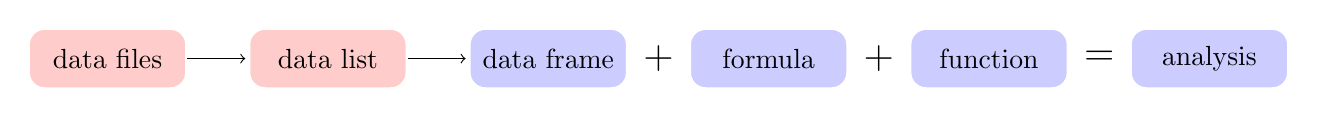
\begin{tikzpicture} [
	node distance=0cm,
	stand/.style={
		rectangle,draw=blue!0,fill=blue!20,thick,
		rounded corners=2mm,
		minimum width=2cm},
	new/.style={
		rectangle,draw=red!0,fill=red!20,thick,
		rounded corners=2mm,
		minimum width=2cm},
	otpt/.style={
		rectangle,draw=blue!0,fill=blue!20,thick,
		rounded corners=2mm,
		minimum width=2cm},
	plus/.style={
		rectangle,draw=blue!0,fill=blue!0},
	tip/.style={
		->,shorten >=1pt}]
\node [place,new]	(data files) 				{data files};
\node [place,plus]	(blank1) [right=of data files]	{};
\node [place,new]	(data list) [right=of blank1] 	{data list};
\node [place,plus]	(blank1) [right=of data list]		{};
\node [place,stand]	(data frame) [right=of blank1] 	{data frame};
\node [place,plus]	(plus1) [right=of data frame]	{\Large +};
\node [place,stand]	(formula) [right=of plus1]		{formula};
\node [place,plus]	(plus2) [right=of formula]		{\Large +};
\node [place,stand]	(function) [right=of plus2]		{function};
\node [place,plus]	(equal) [right=of function]		{\Large =};
\node [place,otpt]	(analysis) [right=of equal]		{analysis};
\draw[tip] (data list.east) -- (data frame.west);
\draw[tip] (data files.east) -- (data list.west);
\end{tikzpicture}
\caption{The \pkg{multitable} paradigm for including multiple-table data (in red) into standard \R\ workflows (in blue).  Data lists are used to organise and manipulate multiple-table data as a single \R\ object, even though such data will typically be originally stored in multiple text-based data files.  When such data are ready for analysis, they are coerced into a data frame.  Once in data frame form, they can be used in analyses by combining them with formulas (to specify hypothetical relationships between variables) and functions (to call statistical methods).} 
\label{fig:model}
\end{figure*}

How can data lists make data organisation easier?  Although practically any data set can be forced into a single \code{data.frame} by either repeating some of the data or adding missing values, other structures often exist that would make a particular data set easier to understand, manipulate, and analyse.  Accordingly, we have designed \code{data.list} objects to provide a richer structure than \code{data.frame} objects for representing our data `as we understand them'.  As we have discussed, there are important advantages to organising data in \code{data.frame} objects---perhaps the most important advantage being the powerful catalogue of \R\ functions that accept data in such a form.  The \pkg{multitable} package provides methods for coercing \code{data.list} objects into \code{data.frame} objects, thus making standard \R\ tools available to multiple-table data organised as a \code{data.list} object.  In summary, the \pkg{multitable} model of data organisation is to manipulate, transform, and extract subsets of our data in \code{data.list}-form, and then to coerce them into \code{data.frame}-form when we are ready to pass them to analysis functions (Fig. \ref{fig:model}).  Importantly, data, formulas, and functions are kept separate, thus preserving the benefits of using \R\ in the standard way.

There are several existing \R\ packages that are designed to make data organisation easier (e.g. \pkg{reshape2}; \citeauthor{Wickham2007}, \citeyear{Wickham2007}).  In fact, the \pkg{mefa} and \pkg{mefa4} packages have been developed to organise data with a slight generalisation\footnote{Several community matrices---called segments---with identical dimensions are allowed in \pkg{mefa}.} of the fourth-corner problem \citep{Solymos2009}.  The \pkg{multitable} package has much in common with \pkg{mefa}, but there are noticeable differences.  For example, \pkg{multitable} is designed to handle more general data structures than \pkg{mefa} or \pkg{mefa4}; in particular, \pkg{mefa} is not able to represent the relational structure of the Lac Croche data depicted in Fig. \ref{fig:beatrix}).  On the other hand, \pkg{mefa} provides more extensive tools for data summarisation than \pkg{multitable} and \pkg{mefa4} integrates tools for sparse-matrix computations.  We therefore expect \pkg{mefa} and \pkg{multitable} to often be complementary in practice.

The purpose of this article is to justify and introduce the use of the \pkg{multitable} package.  We begin by describing the structure of a toy \code{data.list} object.  Then we illustrate one of the most powerful features of \code{data.list} objects:  methods that allow related variables, which do not easily fit into a single data frame, to be subscripted simultaneously.  Next we show that variables in data lists can be transformed and modelled, in much the same manner that is standard for variables in data frames.  Finally, we describe a simple method for creating \code{data.list} objects, and use this method to introduce some helpful concepts associated with multiple-table data in general.

\section{The structure of data lists}

The \pkg{multitable} package comes with a fictitious \code{data.list}, to illustrate how these objects work.
\begin{Schunk}
\begin{Sinput}
> library(multitable)
> data(fake.community)
> fake.community
\end{Sinput}
\begin{Soutput}
abundance:
---------
, , capybara

            2009 2008 1537
midlatitude    4    0    0
subtropical    0   10    0
tropical       8    0    0
equatorial     0    7    0
arctic         0    0    0
subarctic      0    0    0

, , moss

            2009 2008 1537
midlatitude    0    6    0
subtropical    0    0    0
tropical       9    0    0
equatorial     0    3    0
arctic         5    0    0
subarctic      0    0    0

, , vampire

            2009 2008 1537
midlatitude    0    0    0
subtropical    0    0    1
tropical       0    0    0
equatorial     0    0    0
arctic         0    0    0
subarctic      0    0    0

Replicated along:  || sites || years || species || 


temperature:
-----------
            2009 2008 1537
midlatitude   NA   10   NA
subtropical   25   20   NA
tropical      48   50   NA
equatorial    50   30   NA
arctic       -37  -30   NA
subarctic      3    0   NA
Replicated along:  || sites || years || 


precipitation:
-------------
            2009 2008 1537
midlatitude   NA   20   NA
subtropical   99  100   NA
tropical     149  150   NA
equatorial   199  200   NA
arctic        21   20   NA
subarctic     41   40   NA
Replicated along:  || sites || years || 


body.size:
---------
capybara     moss  vampire 
     140       NA      190 
Replicated along:  || species || 


metabolic.rate:
--------------
capybara     moss  vampire 
      20        5        0 
Replicated along:  || species || 


homeotherm:
----------
capybara     moss  vampire 
       Y        N        N 
Levels: N Y
Replicated along:  || species || 


REPLICATION DIMENSIONS: 
  sites   years species 
      6       3       3 
\end{Soutput}
\end{Schunk}

At first sight, this \code{data.list} object looks very different from standard \code{data.frame} objects, but on second look we can see that they are really quite similar.  Just like data frames, data lists are composed of a number of variables---in this case, we have six variables (\code{abundance}; \code{temperature}; \code{precipitation}; \code{body.size}; \code{metabolic.rate}; and \code{homeotherm}) each identified in the printed object above by underlined names.  The variables in data lists must be printed in this sequential manner, rather than as columns neatly lined up in a data frame, precisely because the variables in multiple-table data sets do not line up neatly; this is the problem \pkg{multitable} seeks to address.

Also as with data frames, the replication of variables in data lists are represented as vectors of values.  The main difference between the two objects in this regard is that the vectors that represent variables in data lists have \code{dim} (i.e. dimension) attributes.  These \code{dim} attributes give \code{data.list} objects further structure.  In \R, vectors with \code{dim} attributes are best thought of as matrices and arrays of numbers.  For example, the \code{abundance} variable is replicated along three dimensions (sites; years; and species), and therefore is a three dimensional array of data.  This information is displayed after the data whenever a \code{data.list} object is printed.  Some variables are only replicated along two dimensions (e.g. \code{temperature} and \code{precipitation}) and others only have one dimension (e.g. \code{body.size}; \code{metabolic.rate}; and \code{homeotherm}).  


Importantly however, although the variables are not replicated along all of the same dimensions, they do share dimensions; and it is this dimension sharing that allows us to relate variables to each other.  To appreciate the dimension sharing of this example, we can use the \code{summary} method for \code{data.list} objects:
\begin{Schunk}
\begin{Sinput}
> summary(fake.community)
\end{Sinput}
\begin{Soutput}
        abundance temperature precipitation
sites        TRUE        TRUE          TRUE
years        TRUE        TRUE          TRUE
species      TRUE       FALSE         FALSE
        body.size metabolic.rate homeotherm
sites       FALSE          FALSE      FALSE
years       FALSE          FALSE      FALSE
species      TRUE           TRUE       TRUE
\end{Soutput}
\end{Schunk}
This method returns a logical matrix with dimensions of replication as rows and variables as columns.  A value of \code{TRUE} appears in cells corresponding to variables that are replicated along a particular dimension, and a value of \code{FALSE} appears otherwise.  We can see that the \code{sites} and \code{years} dimensions relate \code{abundance}, \code{temperature}, and \code{precipitation}; whereas, the \code{species} dimension relates \code{abundance}, \code{body size}, \code{metabolic rate}, and \code{homeotherm}.

Note that some \code{FALSE} entries are biophysical necessities, whereas others are properties of the study design.  For example, suppose that later in the study, the researchers decided that it was necessary to get some idea of the spatial variation in metabolic rates.  It would then be possible to measure metabolic rates of the species at different sites, thereby changing the \code{FALSE} associated with the metabolic rate-sites cell to a \code{TRUE}.  To the contrary, it is both physically and logically impossible to measure the precipitation of a species, so this \code{FALSE} is mandatory.

\section{Subscripting data lists}

The structure relating variables and dimensions of replication allows us to manipulate multiple variables simultaneously.  In particular, \pkg{multitable} makes it possible to extract pieces of a data list while maintaining its structure.  For example, examining the data suggests that 1537 might have been an outlying year relative to 2008 and 2009.  We can exclude data from 1537 just as we would with a single \R\ array:
\begin{Schunk}
\begin{Sinput}
> fake.community[,c("2008","2009"),]
\end{Sinput}
\begin{Soutput}
abundance:
---------
, , capybara

            2008 2009
midlatitude    0    4
subtropical   10    0
tropical       0    8
equatorial     7    0
arctic         0    0
subarctic      0    0

, , moss

            2008 2009
midlatitude    6    0
subtropical    0    0
tropical       0    9
equatorial     3    0
arctic         0    5
subarctic      0    0

, , vampire

            2008 2009
midlatitude    0    0
subtropical    0    0
tropical       0    0
equatorial     0    0
arctic         0    0
subarctic      0    0

Replicated along:  || sites || years || species || 


temperature:
-----------
            2008 2009
midlatitude   10   NA
subtropical   20   25
tropical      50   48
equatorial    30   50
arctic       -30  -37
subarctic      0    3
Replicated along:  || sites || years || 


precipitation:
-------------
            2008 2009
midlatitude   20   NA
subtropical  100   99
tropical     150  149
equatorial   200  199
arctic        20   21
subarctic     40   41
Replicated along:  || sites || years || 


body.size:
---------
capybara     moss  vampire 
     140       NA      190 
Replicated along:  || species || 


metabolic.rate:
--------------
capybara     moss  vampire 
      20        5        0 
Replicated along:  || species || 


homeotherm:
----------
capybara     moss  vampire 
       Y        N        N 
Levels: N Y
Replicated along:  || species || 


REPLICATION DIMENSIONS: 
  sites   years species 
      6       2       3 
\end{Soutput}
\end{Schunk}
This command returns the same data list of variables but without the data from 1537.  Note that every variable replicated along the \code{years} dimension is subscripted appropriately, while variables that are not replicated along this dimension are unchanged.  As another example, perhaps we want all of the data from the first three sites, in 1537, for the first species (i.e. capybara).  The following line would produce such a data list:
\begin{Schunk}
\begin{Sinput}
> fake.community[1:3,"1537",1]
\end{Sinput}
\end{Schunk}
Other subscripting commands will typically work as expected.  Type \code{?Extract.data.list} into the \R\ command line for full information on subscripting \code{data.list} objects.

\section{Transforming variables in data lists}


Often we need to transform variables before passing data frames to functions.  This is easily done with variables in data lists as well.  For example, suppose we want to make a $\log(x+1)$ transformation of the abundance data.
\begin{Schunk}
\begin{Sinput}
> fake.community$abundance <- 
   log1p(fake.community$abundance)
> fake.community$abundance
\end{Sinput}
\begin{Soutput}
, , capybara

                2009     2008 1537
midlatitude 1.609438 0.000000    0
subtropical 0.000000 2.397895    0
tropical    2.197225 0.000000    0
equatorial  0.000000 2.079442    0
arctic      0.000000 0.000000    0
subarctic   0.000000 0.000000    0

, , moss

                2009     2008 1537
midlatitude 0.000000 1.945910    0
subtropical 0.000000 0.000000    0
tropical    2.302585 0.000000    0
equatorial  0.000000 1.386294    0
arctic      1.791759 0.000000    0
subarctic   0.000000 0.000000    0

, , vampire

            2009 2008      1537
midlatitude    0    0 0.0000000
subtropical    0    0 0.6931472
tropical       0    0 0.0000000
equatorial     0    0 0.0000000
arctic         0    0 0.0000000
subarctic      0    0 0.0000000

attr(,"subsetdim")
  sites   years species 
   TRUE    TRUE    TRUE 
\end{Soutput}
\end{Schunk}
We note that \code{fake.community} has a lot of missing values, which were useful for illustrating how data lists handle missing values, but will make further illustrations somewhat underwhelming.  We can replace these missing values with `observed' values using the standard logic of \R\ replacement.
\begin{Schunk}
\begin{Sinput}
> fake.community$temperature[,"1537"] <- 
   c(5,10,30,20,-80,-10)	
> fake.community$precipitation[,"1537"] <- 
   c(5,50,75,50,2,7)
> fake.community$body.size["moss"] <- 1
\end{Sinput}
\end{Schunk}


\section{Simple analysis functions}

Data lists can be passed `as is' to many standard functions in \R\ that normally take data frames.  In the next section we explain in more detail why this works, but for now we consider a simple example.  Perhaps we want to explore whether the interaction between body size and temperature has an influence on abundance.  As a first attempt at model building, we fit a linear model using \code{lm}.
\begin{Schunk}
\begin{Sinput}
> lm(abundance ~ body.size*temperature,
 data=fake.community)
\end{Sinput}
\begin{Soutput}
Call:
lm(formula = abundance ~ body.size * temperature, 
    data = fake.community)

Coefficients:
          (Intercept)              body.size  
            4.484e-01             -1.718e-03  
          temperature  body.size:temperature  
            3.634e-03              5.041e-07  
\end{Soutput}
\end{Schunk}
And this works just as well with mixtures of categorical and numerical data.
\begin{Schunk}
\begin{Sinput}
> lm(abundance ~ homeotherm*temperature,
 data=fake.community)
\end{Sinput}
\begin{Soutput}
Call:
lm(formula = abundance ~ homeotherm * temperature, 
    data = fake.community)

Coefficients:
            (Intercept)              homeothermY  
               0.228770                 0.090178  
            temperature  homeothermY:temperature  
               0.001186                 0.007512  
\end{Soutput}
\end{Schunk}
It also works with other `simple' functions, such as \code{rlm} (robust linear model) in the \pkg{MASS} package.
\begin{Schunk}
\begin{Sinput}
> library(MASS)
> rlm(abundance ~ body.size*temperature,
 data=fake.community)
\end{Sinput}
\begin{Soutput}
Call:
rlm(formula = abundance ~ body.size * temperature, 
    data = fake.community)

Converged in 10 iterations

Coefficients:
          (Intercept)             body.size 
         2.606699e-05         -1.076827e-07 
          temperature body.size:temperature 
         3.043212e-07         -8.994997e-10 

Degrees of freedom: 51 total; 47 residual
  (3 observations deleted due to missingness)
Scale estimate: 5.26e-05 
\end{Soutput}
\end{Schunk}
Therefore, in many cases, data lists enter standard \R\ workflows in exactly the same manner as data frames; the advantage of data lists in these cases is that they are represented `as we understand them', and this makes manipulating them easier.

\section{Coercing data lists to data frames}


The reason that unmodified data lists can be passed to some functions that are expecting data frames, is that these functions try to coerce whatever data object they receive into a data frame.  When the \pkg{multitable} package is loaded, these functions can find a method for making such a conversion.  This method can be accessed by users directly via the \code{as.data.frame} function from the \R\ \code{base} package.  For example, we can pass the \code{fake.community} data to \code{as.data.frame}.
\begin{Schunk}
\begin{Sinput}
> fake.community.df <- as.data.frame(fake.community)
\end{Sinput}
\end{Schunk}
\begin{table*}
\caption{The \code{fake.community} \code{data.list} object that has been coerced into a \code{data.frame}.}
\label{tab:dataframe}
\begin{Schunk}
\begin{Soutput}
                          abundance temperature precipitation body.size metabolic.rate homeotherm
midlatitude.2009.capybara 1.6094379          NA            NA       140             20          Y
subtropical.2009.capybara 0.0000000          25            99       140             20          Y
tropical.2009.capybara    2.1972246          48           149       140             20          Y
equatorial.2009.capybara  0.0000000          50           199       140             20          Y
arctic.2009.capybara      0.0000000         -37            21       140             20          Y
subarctic.2009.capybara   0.0000000           3            41       140             20          Y
midlatitude.2008.capybara 0.0000000          10            20       140             20          Y
subtropical.2008.capybara 2.3978953          20           100       140             20          Y
tropical.2008.capybara    0.0000000          50           150       140             20          Y
equatorial.2008.capybara  2.0794415          30           200       140             20          Y
arctic.2008.capybara      0.0000000         -30            20       140             20          Y
subarctic.2008.capybara   0.0000000           0            40       140             20          Y
midlatitude.1537.capybara 0.0000000           5             5       140             20          Y
subtropical.1537.capybara 0.0000000          10            50       140             20          Y
tropical.1537.capybara    0.0000000          30            75       140             20          Y
equatorial.1537.capybara  0.0000000          20            50       140             20          Y
arctic.1537.capybara      0.0000000         -80             2       140             20          Y
subarctic.1537.capybara   0.0000000         -10             7       140             20          Y
midlatitude.2009.moss     0.0000000          NA            NA         1              5          N
subtropical.2009.moss     0.0000000          25            99         1              5          N
tropical.2009.moss        2.3025851          48           149         1              5          N
equatorial.2009.moss      0.0000000          50           199         1              5          N
arctic.2009.moss          1.7917595         -37            21         1              5          N
subarctic.2009.moss       0.0000000           3            41         1              5          N
midlatitude.2008.moss     1.9459101          10            20         1              5          N
subtropical.2008.moss     0.0000000          20           100         1              5          N
tropical.2008.moss        0.0000000          50           150         1              5          N
equatorial.2008.moss      1.3862944          30           200         1              5          N
arctic.2008.moss          0.0000000         -30            20         1              5          N
subarctic.2008.moss       0.0000000           0            40         1              5          N
midlatitude.1537.moss     0.0000000           5             5         1              5          N
subtropical.1537.moss     0.0000000          10            50         1              5          N
tropical.1537.moss        0.0000000          30            75         1              5          N
equatorial.1537.moss      0.0000000          20            50         1              5          N
arctic.1537.moss          0.0000000         -80             2         1              5          N
subarctic.1537.moss       0.0000000         -10             7         1              5          N
midlatitude.2009.vampire  0.0000000          NA            NA       190              0          N
subtropical.2009.vampire  0.0000000          25            99       190              0          N
tropical.2009.vampire     0.0000000          48           149       190              0          N
equatorial.2009.vampire   0.0000000          50           199       190              0          N
arctic.2009.vampire       0.0000000         -37            21       190              0          N
subarctic.2009.vampire    0.0000000           3            41       190              0          N
midlatitude.2008.vampire  0.0000000          10            20       190              0          N
subtropical.2008.vampire  0.0000000          20           100       190              0          N
tropical.2008.vampire     0.0000000          50           150       190              0          N
equatorial.2008.vampire   0.0000000          30           200       190              0          N
arctic.2008.vampire       0.0000000         -30            20       190              0          N
subarctic.2008.vampire    0.0000000           0            40       190              0          N
midlatitude.1537.vampire  0.0000000           5             5       190              0          N
subtropical.1537.vampire  0.6931472          10            50       190              0          N
tropical.1537.vampire     0.0000000          30            75       190              0          N
equatorial.1537.vampire   0.0000000          20            50       190              0          N
arctic.1537.vampire       0.0000000         -80             2       190              0          N
subarctic.1537.vampire    0.0000000         -10             7       190              0          N
\end{Soutput}
\end{Schunk}
\end{table*}



The resulting data frame (Table \ref{tab:dataframe}) contains one column for each variable and one row for each combination of replicates across the three dimensions of replication.  Notice that the row names are automatically generated to be informative about the dimensions of replication that have been collapsed into a single dimension.  Unlike the corresponding data list object, the data frame has redundancy.  For example, because the traits are only replicated along \code{species} there are only three unique trait values, one for each of the three species.  These three values are repeated so that all of the variables can be stored side-by-side in a single data frame.

By storing these data in a single data frame, we can now pass them to any function that accepts data frames.  For example, we can graphically examine the interaction between an environmental variable and a trait using the \code{xyplot} function from the \pkg{lattice} package (Fig. \ref{fig:xyplot}):
\begin{Schunk}
\begin{Sinput}
> library(lattice)
> xyplot(abundance ~ temperature | body.size,
   data=fake.community.df)
\end{Sinput}
\end{Schunk}
This function creates a panel for each distinct value of the \code{body.size} variable, with the values of these body sizes indicated by the vertical stripes in the panel titles (see \code{?xyplot}).  In this case, there would not have been much of an interaction between body size and temperature, because the relationships between temperature and abundance do not appear to vary between panels.
\begin{figure}
\includegraphics{multitable-021}
\caption{An \code{xyplot} of the \code{fake.community} data.}
\label{fig:xyplot}
\end{figure}

On occasion, one may wish to iteratively coerce a sequence of data lists to data frames.  For example, in a randomisation test one might loop over a number of random subscripts of a data list.  In such a case, one may find that such an iterative procedure takes too long to run.  Fortunately, we can exploit the fact that each replicated data list has the same structure (i.e. the same replication dimensions and variables) to reduce computation times.  In particular, much of the computational effort involved in coercing data lists to data frames can be done once for all data lists with the same structure.  For more on this technique see the help file for \code{data.list.mold} in the \pkg{multitable} package.

\section{How data lists are made}

Up until now we have used an existing \code{data.list} to illustrate the use of the \pkg{multitable} package.  Although there are several ways to create data lists, one way in particular provides a simple framework for understanding the difference between variables and dimensions of replication---an important distinction to understand in order to use \pkg{multitable} effectively.

Consider a data frame of species abundances counted at various sites.
\begin{Schunk}
\begin{Sinput}
> abundance
\end{Sinput}
\begin{Soutput}
        sites  species abundance
1 midlatitude capybara         4
2 subtropical capybara        10
3    tropical capybara         8
4  equatorial capybara         7
5      arctic     moss         5
6 midlatitude     moss         6
7    tropical     moss         9
8  equatorial     moss         3
9 subtropical  vampire         1
\end{Soutput}
\end{Schunk}
We have six sites and three species, but each species is not present at each site and so there are missing site-species combinations.  Related to this \code{abundance} data frame we have a data frame of environmental variables at each site and a data frame of traits for each species.
\begin{Schunk}
\begin{Sinput}
> environment
\end{Sinput}
\begin{Soutput}
        sites temperature precipitation
1   subarctic           0            40
2 midlatitude          10            20
3 subtropical          20           100
4    tropical          50           150
5  equatorial          30           200
\end{Soutput}
\begin{Sinput}
> trait
\end{Sinput}
\begin{Soutput}
   species body.size metabolic.rate
1 capybara       140             20
2     moss         5              5
3  vampire       190              0
\end{Soutput}
\end{Schunk}
To make things interesting to scientists with real data, we assume that our environmental data are missing from the arctic site (perhaps because it is too remote to go there and make measurements).

The three data frames are related because they share two columns:  sites and species.  The specific pattern of sharing for these data can be illustrated with a bipartite graph (i.e. matching diagram; Fig.\ref{fig:bipartite}).  Columns that are shared between data frames are called \emph{dimensions of replication} and those that are not are called \emph{variables}.  The reason for this terminology is that in standard single-table statistical settings, we are able to relate variables because they are replicated along some common dimension.  For example, one can relate pH and temperature if they are both replicated along the same set of lakes.  Similarly, we can relate the variables in several tables together if they share columns (i.e. dimensions of replication).

\begin{figure}
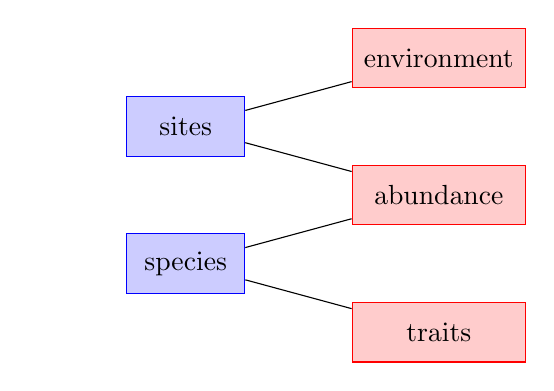
\begin{tikzpicture} [
	text centered,
	node distance=0.1cm,
	ndims/.style={
		rectangle,minimum width=1.5cm,draw=blue!=0,
		fill=blue!20
	},
	nvars/.style={
		rectangle,minimum width=2.2cm,draw=red!=0,
		fill=red!20
	},
	nblank/.style={
		rectangle,draw=red!=0,fill=red!0,draw opacity=0,
		minimum width=4cm
	}
]
\node [place,nblank]	(asites)					{};
\node [place,ndims]	(sites)[below=of asites]		{sites};
\node [place,nblank]	(bsites)[below=of sites]		{};
\node [place,ndims]	(species)[below=of bsites]		{species};
\node [place,nblank]	(bspecies)[below=of species]	{};
\node [place,nvars]	(environment)[right=of asites]	{environment}
	edge [-]		(sites);
\node [place,nvars]	(abundance)[right=of bsites]	{abundance}
	edge [-]		(sites)
	edge [-]		(species);
\node [place,nvars]	(traits)[right=of bspecies]		{traits}
	edge [-]		(species);
\end{tikzpicture}
\caption{Bipartite graph of the multiple-table structure of data with a standard fourth-corner structure (Fig. \ref{fig:fourth}).  Dimensions of replication are in blue (on the left) and tables are in red (on the right).}
\label{fig:bipartite}
\end{figure}

To create a data list out of these data frames we use the \code{dlcast} function from \pkg{multitable}, which was inspired by the \code{acast} function in the \pkg{reshape2} package \citep{Wickham2007}.
\begin{Schunk}
\begin{Sinput}
> dl <- dlcast(list(abundance,environment,trait),
 	dimids=c("sites","species"),
 	fill=c(0,NA,NA)
 )
> dl
\end{Sinput}
\begin{Soutput}
abundance:
---------
            capybara moss vampire
arctic             0    5       0
equatorial         7    3       0
midlatitude        4    6       0
subtropical       10    0       1
tropical           8    9       0
subarctic          0    0       0
Replicated along:  || sites || species || 


temperature:
-----------
     arctic  equatorial midlatitude 
         NA          30          10 
subtropical    tropical   subarctic 
         20          50           0 
Replicated along:  || sites || 


precipitation:
-------------
     arctic  equatorial midlatitude 
         NA         200          20 
subtropical    tropical   subarctic 
        100         150          40 
Replicated along:  || sites || 


body.size:
---------
capybara     moss  vampire 
     140        5      190 
Replicated along:  || species || 


metabolic.rate:
--------------
capybara     moss  vampire 
      20        5        0 
Replicated along:  || species || 


REPLICATION DIMENSIONS: 
  sites species 
      6       3 
\end{Soutput}
\end{Schunk}
This function takes three arguments:  (1) a list of data frames, (2) a character vector, \code{dimids}, with the names identifying the dimensions of replication (i.e. the names of the columns shared between the tables), and (3) a vector, \code{fill}, with one element for each data frame giving the value with which to fill in any structural missing values.  This last argument is interesting because we can both (1) fill missing abundances with zeros because those site-species combinations were not observed and (2) fill missing traits and environmental variables with \code{NA} values.

Researchers will often have text files or spreadsheets of data that are not stored in the same format as the three data frames in our example.  Our three data frames have two types of columns---some columns represent dimensions of replication and others represent variables.  This data storage format is sometimes called `long format' (see \code{?reshape}), because more sampling results in a lengthening of the data (i.e. the addition of rows) without any widening (i.e. the addition of columns).  In contrast, it is common in community ecology for example to store abundance data as spreadsheets with sites as rows and species as columns (e.g. as in Fig \ref{fig:fourth}).  Such a data storage format is often called `wide format', because more sampling may result in a widening of the data (e.g. more columns are required as further sampling reveals a greater diversity of species).  Fortunately, the \pkg{multitable} package provides tools for reading data stored in a variety of different formats into a data list.  For example, the \code{as.data.list}, \code{data.list}, \code{read.multitable}, and \code{read.fourthcorner} functions are all alternatives to \code{dlcast} for creating data lists.

\section{Multiple-table concepts}

The \pkg{multitable} package is based on a distinction between dimensions of replication and variables.  One benefit of this distinction is that it provides a common framework for understanding both simple and more complex multiple-table data structures.  In particular, the framework allows us to visualise the structure of complex data; for example the Lac Croche zooplankton community data (Fig. \ref{fig:beatrix}) \citep{CantinEtAl2011} has a structure given by Fig. \ref{fig:bipartitebeatrix}.  To store these data in a format amenable to \code{dlcast} (i.e. `long format'), we would create one data frame for each of the groups of variables (red boxes on the right) and add a column for each dimension of replication (blue boxes on the left) associated with those variables.

\begin{figure}
\vspace{0.1cm}
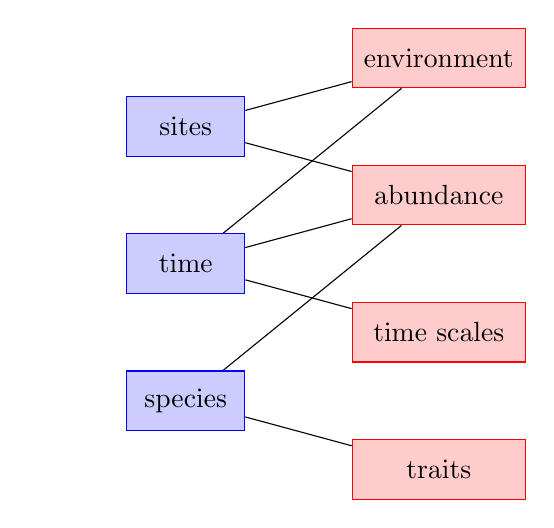
\begin{tikzpicture} [
	text centered,
	node distance=0.1cm,
	ndims/.style={
		rectangle,minimum width=1.5cm,draw=blue!=0,
		fill=blue!20
	},
	nvars/.style={
		rectangle,minimum width=2.2cm,draw=red!=0,
		fill=red!20
	},
	nblank/.style={
		rectangle,draw=red!=0,fill=red!0,draw opacity=0,
		minimum width=4cm
	}
]
\node [place,nblank]	(asites)					{};
\node [place,ndims]	(sites)[below=of asites]		{sites};
\node [place,nblank]	(bsites)[below=of sites]		{};
\node [place,ndims]	(time)[below=of bsites]		{time};
\node [place,nblank]	(btime)[below=of time]		{};
\node [place,ndims]	(species)[below=of btime]		{species};
\node [place,nblank]	(bspecies)[below=of species]	{};
\node [place,nvars]	(environment)[right=of asites]	{environment}
	edge [-]		(sites)
	edge [-]		(time);
\node [place,nvars]	(abundance)[right=of bsites]	{abundance}
	edge [-]		(sites)
	edge [-]		(time)
	edge [-]		(species);
\node [place,nvars]	(scales)[right=of btime]		{time scales}
	edge [-]		(time);
\node [place,nvars]	(traits)[right=of bspecies]		{traits}
	edge [-]		(species);
\end{tikzpicture}
\caption{Bipartite graph of the Lac Croche data in Fig. \ref{fig:beatrix}.} 
\label{fig:bipartitebeatrix}
\end{figure}

Visualising the structure of data in this way will help to clarify how it should be both organised and analysed.  One of the central themes of \pkg{multitable} is that thinking about data organisation goes a long way towards clarifying how analysis should proceed.  The names of what we store as variables will appear in formula objects, so that we can study the relationships between these variables.  On the other hand, the information that we have for inferring these relationships will come from what we store as dimensions of replication.  In single-table settings we keep these two elements of data analysis separate by storing variables as columns and replicates as rows in a \code{data.frame}.  The \code{data.list} concept is very similar except that replication now has a dimensionality, which allows for the storage of more complex data structures.  The basic distinction between variables and replicates guides analysis in multiple-table settings just as it does in single-table settings.

The two requirements for using \code{data.list} objects are that (1) every table must share at least one dimension of replication with at least one other table and (2) at least one table must be replicated along all of the dimensions present in the data set.  The first criterion ensures that the tables will relate to each other; the second criterion ensures that some variables will be relatable to all other variables, a property that is necessary for a response variable.

\section{Conclusion}

The structure of \code{data.list} objects is sufficiently rich to give rise to a much wider variety of uses than can be described in detail here.  Our intention was to illustrate the basic features and concepts of the \pkg{multitable} package, and to demonstrate its utility.  Our long-term goal with the \pkg{multitable} project in general is to make standard analyses in \R\ simpler to conduct on complex multiple-table data.

\section*{Acknowledgements}
We thank Levi Waldron, Ben Bolker, and Philip Dixon for discussions and suggestions about software design and Beatrix Beisner for discussions about biology.

\bibliographystyle{abbrvnat}
\bibliography{Bibliography}

\end{article}
\end{document}
